\documentclass[a0paper,landscape]{baposter}

\usepackage{textcomp}
% \usepackage[T1]{fontenc}
\usepackage[utf8]{inputenc}
\usepackage{tgheros}
% \usepackage{tgbonum}
% \renewcommand*\familydefault{\sfdefault}
% \setmainfont{Arial}
\renewcommand{\familydefault}{\sfdefault}

\usepackage{calc}
\usepackage{amsmath}
\usepackage{amssymb}
\usepackage{mathtools}
\usepackage{relsize}
\usepackage{multirow}
\usepackage{bm}
\usepackage{enumitem}

%\usepackage{amsfonts}
%\usepackage{cmbright}
%\usepackage{comicsans}
\usepackage[cm]{sfmath}


\usepackage{graphicx}
\usepackage{multicol}

\pgfdeclarelayer{background}
\pgfdeclarelayer{foreground}
\pgfsetlayers{background,main,foreground}

\usepackage{tikz,pgfplots,pgfplotstable,gnuplot-lua-tikz}

\usetikzlibrary{shapes,arrows,decorations.markings,shadows,positioning}
% \usepackage{helvet}
%\usepackage{bookman}
%\usepackage{palatino}
\usepackage{enumitem}
\usepackage{tensor}
\newcommand\Perms[2]{\tensor[_{#1}]P{_{#2}}}
\newcommand{\captionfont}{\footnotesize}

\usepackage[vlined,titlenotnumbered]{algorithm2e}
\usepackage{minibox}
\usepackage{listings}
% Define custom style for AMPL code listings
\lstdefinelanguage{AMPL}{keywords={set,param,var,arc,integer,minimize,maximize,subject,to,node,
sum,in,Current,complements,integer,solve_result_num,IN,contains,less,suffix,INOUT,default,logical,
Infinity,dimen,max,symbolic,Initial,div,min,table,LOCAL,else,option,then,OUT,environ,setof,union,
all,exists,shell_exitcodeuntil,binary,forall,solve_exitcodewhile,by,if,solve_messagewithin,check,
solve_result,true,false,include},sensitive=true,comment=[l]{\#}}
\lstdefinestyle{AMPL}{
	language=AMPL,
	aboveskip=3mm,
	belowskip=3mm,
	showstringspaces=false,
	columns=flexible,
        %	keywordstyle=\bfseries,
        keywordstyle=\color{ArgonneLogoRed},
	breaklines=true,
	breakatwhitespace=true,
	tabsize=3,
}
% Define custom style for Python code listings
\definecolor{codegreen}{rgb}{0,0.6,0}
\definecolor{backcolour}{rgb}{0.95,0.95,0.92}
\lstdefinestyle{python}{
    language=python,
    numbers=none,
    backgroundcolor=\color{backcolour},
    commentstyle=\color{blue},
    keywordstyle=\color{magenta},
    stringstyle=\color{codegreen},
    basicstyle=\ttfamily\footnotesize,
    breakatwhitespace=false,
    breaklines=true,
    captionpos=b,
    keepspaces=true,
    showspaces=false,
    showstringspaces=false,
    showtabs=false,
    tabsize=3
}
\usepackage{tcolorbox}

\let\oldnl\nl% Store \nl in \oldnl
\newcommand{\nonl}{\renewcommand{\nl}{\let\nl\oldnl}}% Remove line number for one line

\renewcommand{\emph}{\textbf}

\graphicspath{{./images/}}
\setlist[itemize]{leftmargin=*}
\setlist[enumerate]{leftmargin=*}

%%%%%%%%%%%%%%%%%%%%%%%%%%%%%%%%%%%%%%%%%%%%%%%%%%%%%%%%%%%%%%%%%%%%%%%%%%%%%%%%
%%%% Some math symbols used in the text
%%%%%%%%%%%%%%%%%%%%%%%%%%%%%%%%%%%%%%%%%%%%%%%%%%%%%%%%%%%%%%%%%%%%%%%%%%%%%%%%
% Format 
\newcommand{\cR}{\mathcal{R}_S} 		% Random stream
\newcommand{\cQ}{Q_L} 	          	% Localopt Queue

\newcommand{\R}{\mathbb{R}}  % The reals
\newcommand{\cW}{\mathcal{W}} 	% Workers
\newcommand{\cD}{\mathcal{D}} 		% Box-constrained domain
\newcommand{\nw}{n_\mathcal{W}} 	% Number of workers
\newcommand{\tn}{\textnormal}
\newcommand{\maximize}{\operatornamewithlimits{maximize}}
\newcommand{\minimize}{\operatornamewithlimits{minimize}}
\newcommand{\mins}{\operatornamewithlimits{min}}
\newcommand{\argmax}{\operatornamewithlimits{argmax}}
\newcommand{\argmin}{\operatornamewithlimits{argmin}}
\newcommand{\fGamma}{\operatorname{\Gamma}}
\newcommand{\floor}[1] {\lfloor #1 \rfloor}
\newcommand{\ceil}[1] {\lceil #1 \rceil}
\newcommand{\vol}[1] {\operatorname{vol}\left( #1 \right)}
\newcommand{\BigO}[1]{\ensuremath{\operatorname{O}\bigl(#1\bigr)}}
\newcommand{\Matrix}[1]{\begin{bmatrix} #1 \end{bmatrix}}
\newcommand{\Vector}[1]{\Matrix{#1}}

\newcommand*{\SET}[1]  {\ensuremath{\mathcal{#1}}}
\newcommand*{\MAT}[1]  {\ensuremath{\mathbf{#1}}}
\newcommand*{\VEC}[1]  {\ensuremath{\bm{#1}}}
\newcommand*{\CONST}[1]{\ensuremath{\mathit{#1}}}
\newcommand*{\norm}[1]{\mathopen\| #1 \mathclose\|}% use instead of $\|x\|$
\newcommand*{\abs}[1]{\mathopen| #1 \mathclose|}% use instead of $\|x\|$
\newcommand*{\absLR}[1]{\left| #1 \right|}% use instead of $\|x\|$

\def\norm#1{\mathopen\| #1 \mathclose\|}% use instead of $\|x\|$
\newcommand{\normLR}[1]{\left\| #1 \right\|}% use instead of $\|x\|$

% Argonne Logo Colors
\definecolor{ArgonneLogoBlue}{RGB}{4,146,210}
\definecolor{ArgonneLiteBlue}{RGB}{202,214,246}%{176,196,222}
\definecolor{ArgonneLogoRed}{RGB}{228,32,41}
\definecolor{ArgonneLogoGreen}{RGB}{120,202,42}
\definecolor{PMSCoolGray}{RGB}{112,109,110}


\newcommand{\BLUE}[1]{\textcolor{blue}{\bf #1}}
\newcommand{\RED}[1]{\textcolor{ArgonneLogoRed}{\bf #1}}
\newcommand{\PURPLE}[1]{\textcolor{purple}{\bf #1}}
\newcommand{\GREEN}[1]{\textcolor{ArgonneLogoGreen}{\bf #1}}

%%%%%%%%%%%%%%%%%%%%%%%%%%%%%%%%%%%%%%%%%%%%%%%%%%%%%%%%%%%%%%%%%%%%%%%%%%%%%%%%
% Multicol Settings
%%%%%%%%%%%%%%%%%%%%%%%%%%%%%%%%%%%%%%%%%%%%%%%%%%%%%%%%%%%%%%%%%%%%%%%%%%%%%%%%
\setlength{\columnsep}{0.7em}
\setlength{\columnseprule}{0mm}


%%%%%%%%%%%%%%%%%%%%%%%%%%%%%%%%%%%%%%%%%%%%%%%%%%%%%%%%%%%%%%%%%%%%%%%%%%%%%%%%
% Save space in lists. Use this after the opening of the list
%%%%%%%%%%%%%%%%%%%%%%%%%%%%%%%%%%%%%%%%%%%%%%%%%%%%%%%%%%%%%%%%%%%%%%%%%%%%%%%%
\newcommand{\compresslist}{%
\setlength{\itemsep}{1pt}%
\setlength{\parskip}{0pt}%
\setlength{\parsep}{0pt}%
}

\newcommand{\alert}{\RED}
\newcommand{\X}{{\cal X}}
\newcommand{\U}{{\cal U}}
\newcommand{\RA}{$\Rightarrow$}
\newcommand{\ra}{\alert{a}}

\newcommand{\mini}{\mathop{\mbox{minimize}}}
\newcommand{\maxi}{\mathop{\mbox{maximize}}}
\newcommand{\st}{\mbox{subject to}}
\newcommand{\stn}{\mbox{s.t.}}
\newcommand{\dps}{\displaystyle}
\newcommand{\readers}[1]{}

%%%%%%%%%%%%%%%%%%%%%%%%%%%%%%%%%%%%%%%%%%%%%%%%%%%%%%%%%%%%%%%%%%%%%%%%%%%%%%
%%% Begin of Document
%%%%%%%%%%%%%%%%%%%%%%%%%%%%%%%%%%%%%%%%%%%%%%%%%%%%%%%%%%%%%%%%%%%%%%%%%%%%%%

\begin{document}

%%%%%%%%%%%%%%%%%%%%%%%%%%%%%%%%%%%%%%%%%%%%%%%%%%%%%%%%%%%%%%%%%%%%%%%%%%%%%%
%%% Here starts the poster
%%%---------------------------------------------------------------------------
%%% Format it to your taste with the options
%%%%%%%%%%%%%%%%%%%%%%%%%%%%%%%%%%%%%%%%%%%%%%%%%%%%%%%%%%%%%%%%%%%%%%%%%%%%%%
\typeout{Poster Starts}
\background{
  \begin{tikzpicture}[remember picture,overlay]%
    \draw (current page.north west)+(-2em,-0em) node[anchor=north west] {\hspace{-2em}\includegraphics[height=1.1\textheight]{silhouettes_background}};
  \end{tikzpicture}%
}
\definecolor{silver}{cmyk}{0,0,0,0.3}
\definecolor{yellow}{cmyk}{0,0,0.9,0.0}
\definecolor{reddishyellow}{cmyk}{0,0.22,1.0,0.0}
\definecolor{black}{cmyk}{0,0,0.0,1.0}
\definecolor{darkYellow}{cmyk}{0,0,1.0,0.5}
\definecolor{darkSilver}{cmyk}{0,0,0,0.1}

\definecolor{lightyellow}{cmyk}{0,0,0.3,0.0}
\definecolor{lighteryellow}{cmyk}{0,0,0.1,0.0}
\definecolor{lighteryellow}{cmyk}{0,0,0.1,0.0}
\definecolor{lightestyellow}{cmyk}{0,0,0.05,0.0}

\definecolor{KTHBlue}{cmyk}{.71,.37,0.07,0}
\definecolor{KTHsilver}{cmyk}{0,0,0,0.35}
\definecolor{KTHbeige}{cmyk}{0,0.03,0.19,0.04}

% \definecolor{KTHBlue}{RGB}{25,84,166}
\begin{poster}{
  % Show grid to help with alignment
  grid=false,
  columns=3,
  % Column spacing
  colspacing=1em,
  % Color style
  % bgColorOne=ArgonneLogoRed,
  bgColorOne=white,
  bgColorTwo=white,
  borderColor=PMSCoolGray,
  headerColorOne=ArgonneLiteBlue,
  headerColorTwo=ArgonneLogoBlue,
  headerFontColor=black,
  boxColorOne=white,
  boxColorTwo=white,
  % Format of textbox
  textfont=\large,
  textborder=roundedleft,
  % Format of text header
  eyecatcher=true,
  headerborder=open,
  % headerheight=0.08\textheight,
  headerheight=0.14\textheight,
  headershape=roundedright,
  headershade=plain,
%  headershade=shade-lr,
  headerfont=\Large\sf\bf, %Sans Serif
  boxshade=plain,
%  background=shade-tb,
  background=plain,
  linewidth=2pt
  }
  % Eye Catcher
  {
\includegraphics[height=6em]{../img/logos/Argonne_cmyk_black.eps}} % No eye catcher for this poster. If an eye catcher is present, the title is centered between eye-catcher and logo.
  % Title
  {\sf $\quad$\\A framework for fully autonomous design of materials via multiobjective optimization and active learning\\$\quad$}
  % Authors
  {\sf  \phantom{\hspace{0em}}
    Tyler Chang$^1$, Jakob Elias$^1$, Stefan Wild$^2$, Santanu Chaudhuri$^{1,3}$ and Joseph Libera$^1$\\

    \smallskip

    {\it \small
    $^1$Argonne National Laboratory $\quad$
    $^2$Lawrence Berkeley National Laboratory $\quad$
    $^3$University of Illinois Chicago\\
    \par
    }

  }
  % Top right logo
  {
    
\includegraphics[height=4em]{../img/logos/DOE_logo_color_cmyk.eps}
  }

  \tikzstyle{light shaded}=[top color=baposterBGtwo!30!white,bottom color=baposterBGone!30!white,shading=axis,shading angle=30]

  % Width of left inset image
 \newlength{\leftimgwidth}
 \setlength{\leftimgwidth}{0.78em+8.0em}
 
 \newcounter{boxnum}
 \newcommand{\thebox}{\stepcounter{boxnum} \arabic{boxnum}. }

%%%%%%%%%%%%%%%%%%%%%%%%%%%%%%%%%%%%%%%%%%%%%%%%%%%%%%%%%%%%%%%%%%%%%%%%%%%%%%
%%% Now define the boxes that make up the poster
%%%---------------------------------------------------------------------------
%%% Each box has a name and can be placed absolutely or relatively.
%%% The only inconvenience is that you can only specify a relative position 
%%% towards an already declared box. So if you have a box attached to the 
%%% bottom, one to the top and a third one which should be in between, you 
%%% have to specify the top and bottom boxes before you specify the middle 
%%% box.
%%%%%%%%%%%%%%%%%%%%%%%%%%%%%%%%%%%%%%%%%%%%%%%%%%%%%%%%%%%%%%%%%%%%%%%%%%%%%%
  %
  % A coloured circle useful as a bullet with an adjustably strong filling
  \newcommand{\colouredcircle}[1]{%
    \tikz{\useasboundingbox (-0.2em,-0.32em) rectangle(0.2em,0.32em); \draw[draw=black,fill=baposterBGone!80!black!#1!white,line width=0.03em] (0,0) circle(0.18em);}}

%%%%%%%%%%%%%%%%%%%%%%%%%%%%%%%%%%%%%%%%%%%%%%%%%%%%%%%%%%%%%%%%%%%%%%%%%%%%%%
\headerbox{Our (Big) Goals}{name=goals,column=0,row=0}{
%%%%%%%%%%%%%%%%%%%%%%%%%%%%%%%%%%%%%%%%%%%%%%%%%%%%%%%%%%%%%%%%%%%%%%%%%%%%%%
  \setlength{\parskip}{0.5\baselineskip}

  \smallskip

  {\small
  \begin{itemize}
  \item Design a software framework for {\sl self-driving labs}
  \item Accelerate discovery via intelligent experimentation
  \item Democratize lab-work by building open-source tools
  \end{itemize}}
}

%%%%%%%%%%%%%%%%%%%%%%%%%%%%%%%%%%%%%%%%%%%%%%%%%%%%%%%%%%%%%%%%%%%%%%%%%%%%%%
\headerbox{Streaming data from multiple sources}{name=mdml,column=0,below=goals}{
%%%%%%%%%%%%%%%%%%%%%%%%%%%%%%%%%%%%%%%%%%%%%%%%%%%%%%%%%%%%%%%%%%%%%%%%%%%%%%
  \setlength{\parskip}{0.5\baselineskip}

  \smallskip

  {\small
  \begin{itemize}
  \item How to collect and analyze data?
  \item MDML is a platform for streaming, analyzing, and
  logging experiment and simulation data
  \end{itemize}
  }
  \begin{center}
  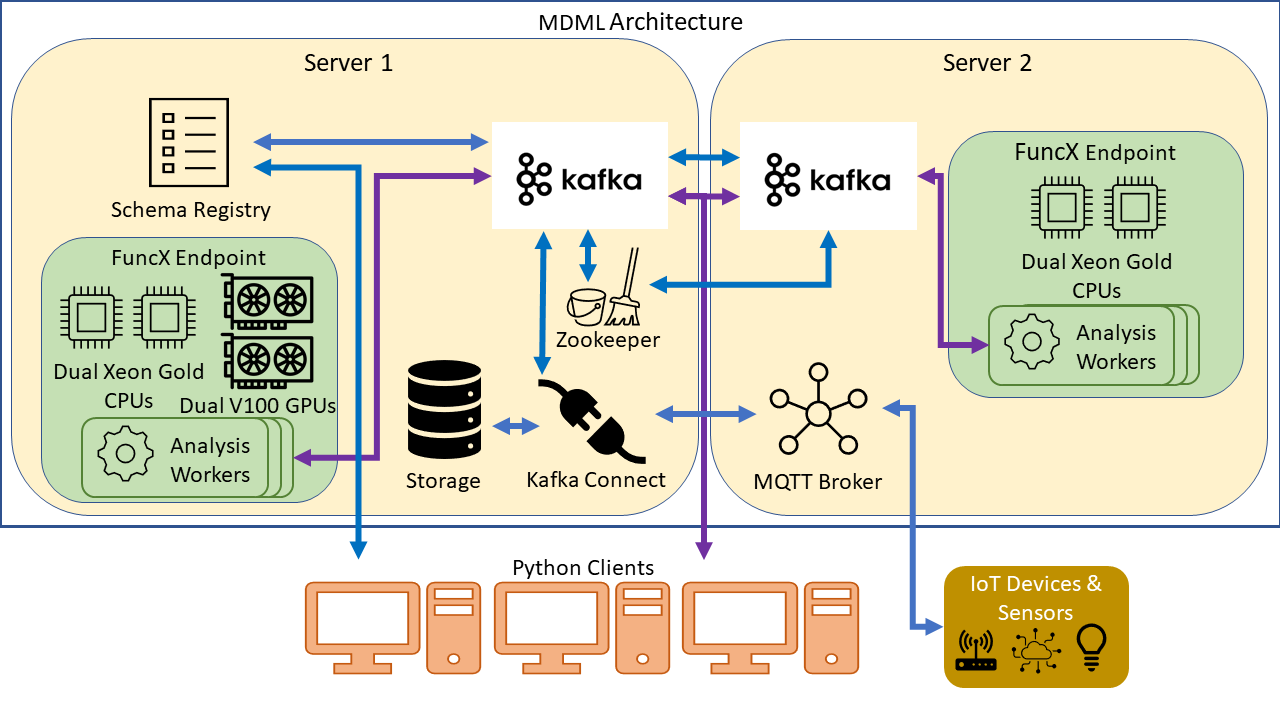
\includegraphics[width=0.85\textwidth]{../img/moo_new/MDML_arch_v2.png}
  \end{center}
}

%%%%%%%%%%%%%%%%%%%%%%%%%%%%%%%%%%%%%%%%%%%%%%%%%%%%%%%%%%%%%%%%%%%%%%%%%%%%%%
\headerbox{Model-based optimization}{name=opt,column=0,below=mdml,above=bottom}{
%%%%%%%%%%%%%%%%%%%%%%%%%%%%%%%%%%%%%%%%%%%%%%%%%%%%%%%%%%%%%%%%%%%%%%%%%%%%%%
  \setlength{\parskip}{0.5\baselineskip}

  \smallskip

  {\small
  \begin{itemize}
  \item ParMOO (multiobjective optimization) library is used to implement an
  active learning loop
  \end{itemize}
  }

  \begin{center}

  \vskip -20pt

  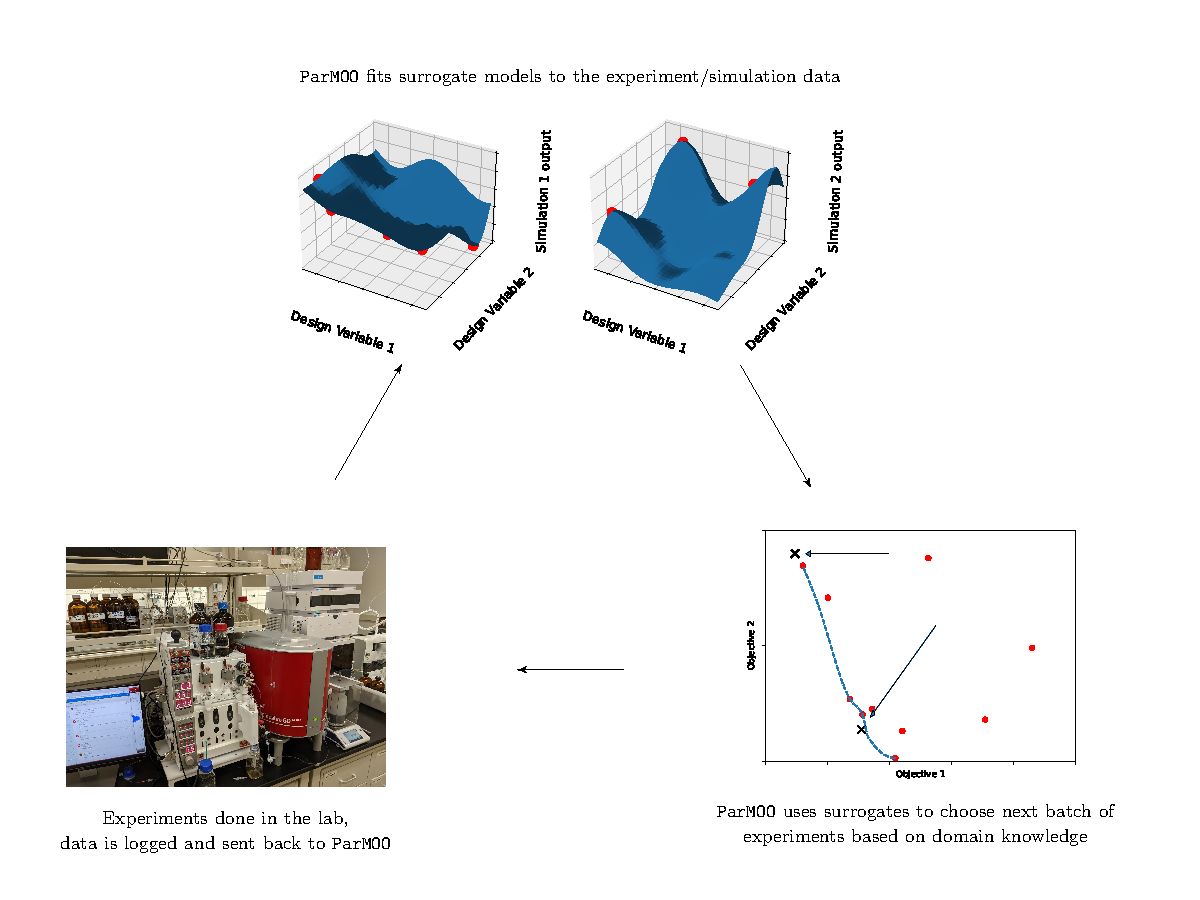
\includegraphics[width=0.89\textwidth]{../img/moo_new/active-learning-loop.pdf}
  \end{center}

}

%%%%%%%%%%%%%%%%%%%%%%%%%%%%%%%%%%%%%%%%%%%%%%%%%%%%%%%%%%%%%%%%%%%%%%%%%%%%%%
\begin{posterbox}[name=framework,column=1,row=0]{Our framework and software stack}
%%%%%%%%%%%%%%%%%%%%%%%%%%%%%%%%%%%%%%%%%%%%%%%%%%%%%%%%%%%%%%%%%%%%%%%%%%%%%%
  \setlength{\parskip}{0.5\baselineskip}

  \smallskip

  {\small
  \begin{itemize}
  \item MDML gives us access to {\sl heterogeneous data from laboratory sources}
  \item ParMOO gives us modular/customizable {\sl modeling, embedding, and solvers}
  \end{itemize}}
  \begin{center}

  \vskip -25pt

  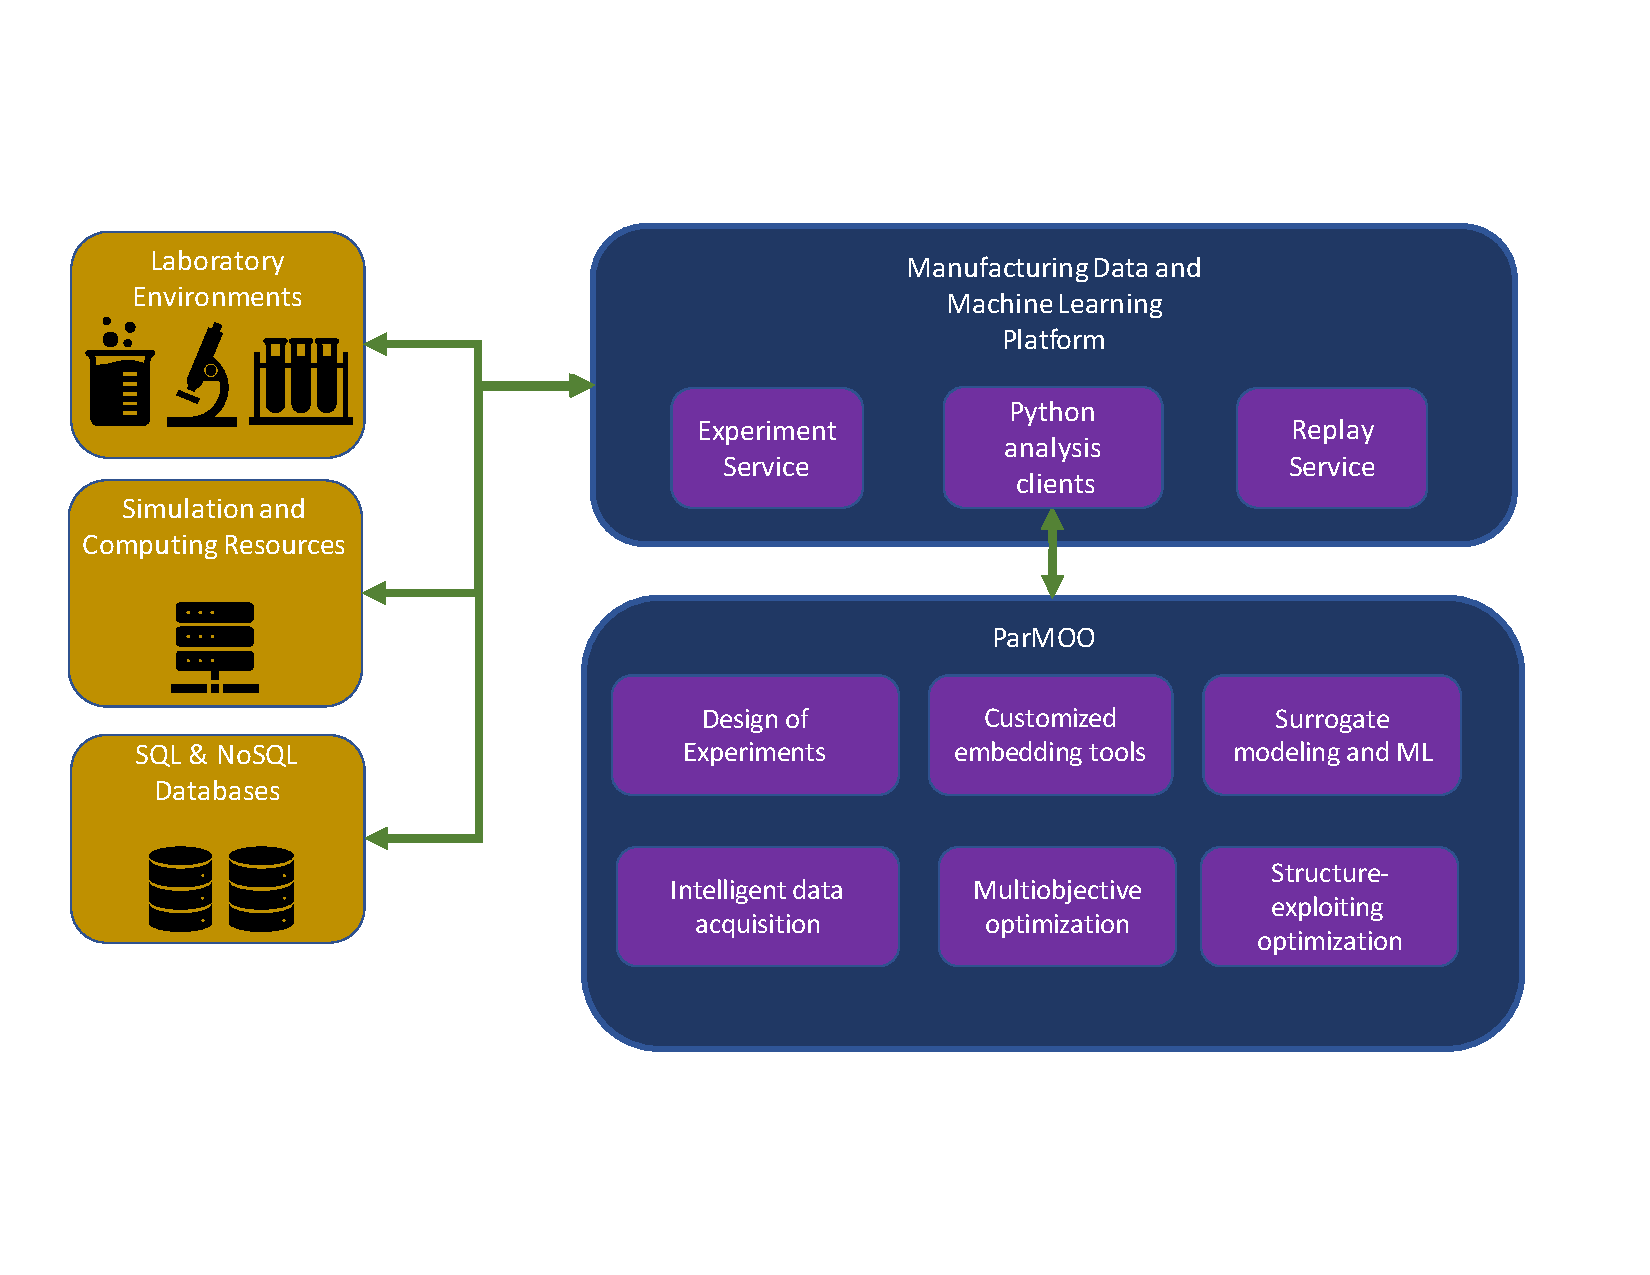
\includegraphics[width=0.8\textwidth]{../img/moo_new/mdml-parmoo-2.pdf}

  \vskip -25pt

  {\small
  Build \& deploy custom solvers for computational and experimental problem!

  }
  \end{center}
\end{posterbox}

%%%%%%%%%%%%%%%%%%%%%%%%%%%%%%%%%%%%%%%%%%%%%%%%%%%%%%%%%%%%%%%%%%%%%%%%%%%%%%
\headerbox{Example: TFMC Manufacturing Conditions}{name=example,column=1,below=framework,above=bottom}{
%%%%%%%%%%%%%%%%%%%%%%%%%%%%%%%%%%%%%%%%%%%%%%%%%%%%%%%%%%%%%%%%%%%%%%%%%%%%%%
  \setlength{\parskip}{0.5\baselineskip}

  \smallskip

  \begin{center}

  {\small
  Optimize the production of TFMC via a known reaction...}

  \vskip -4pt

  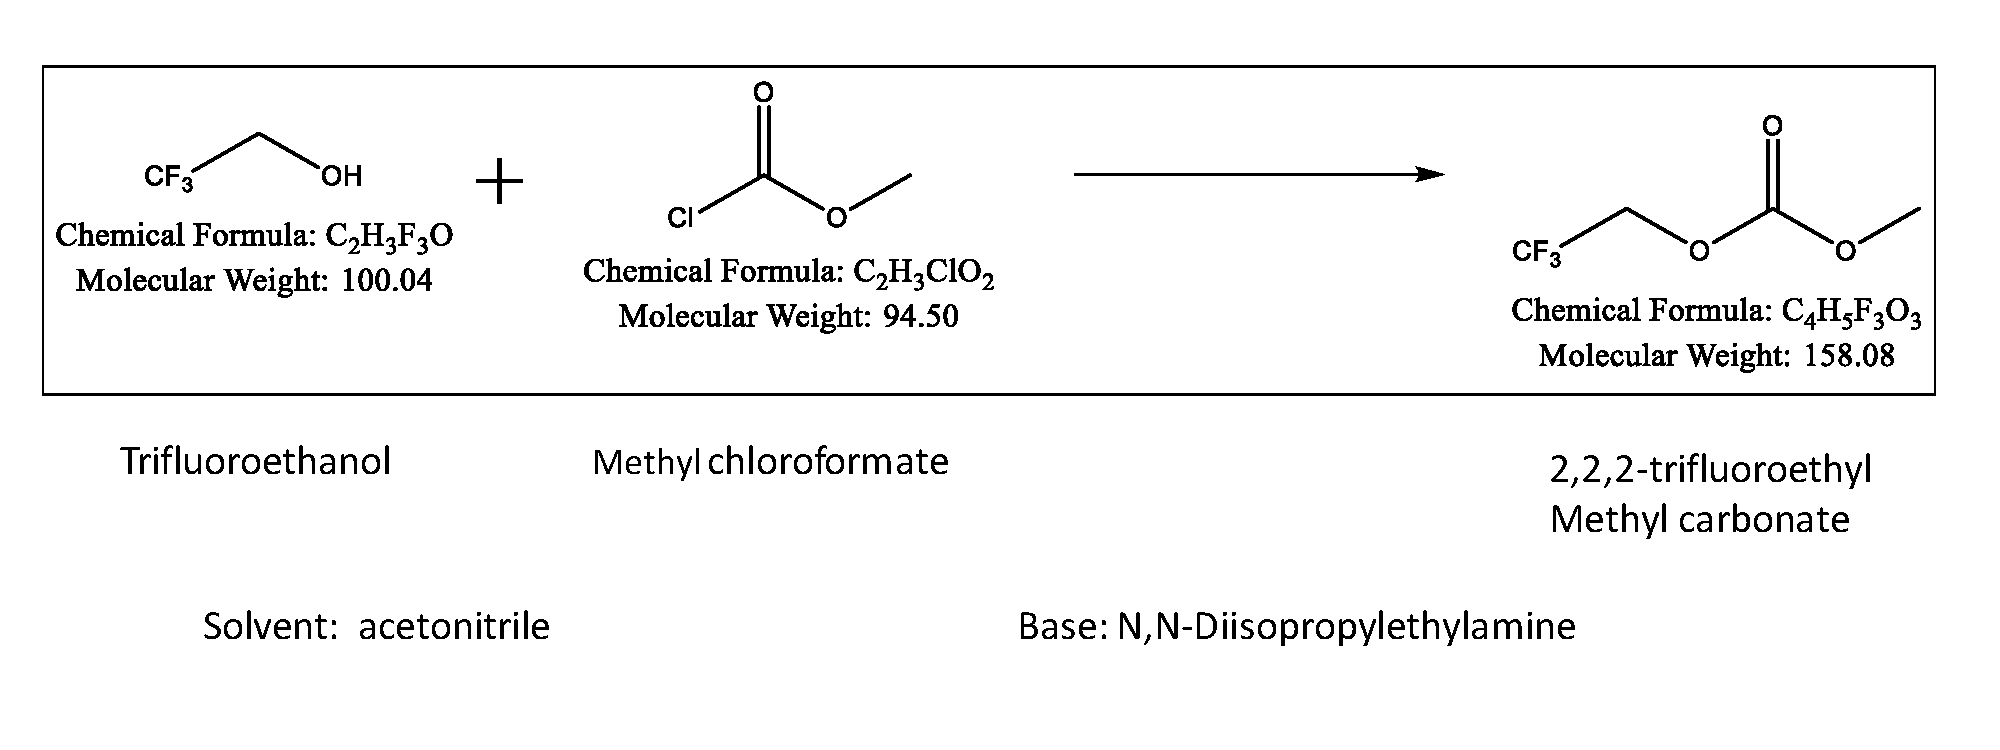
\includegraphics[width=0.8\textwidth]{../img/probs/basic_reaction.pdf}

  \vskip -4pt
  {\small

  \hbox{
   \hskip -70pt
    \vbox{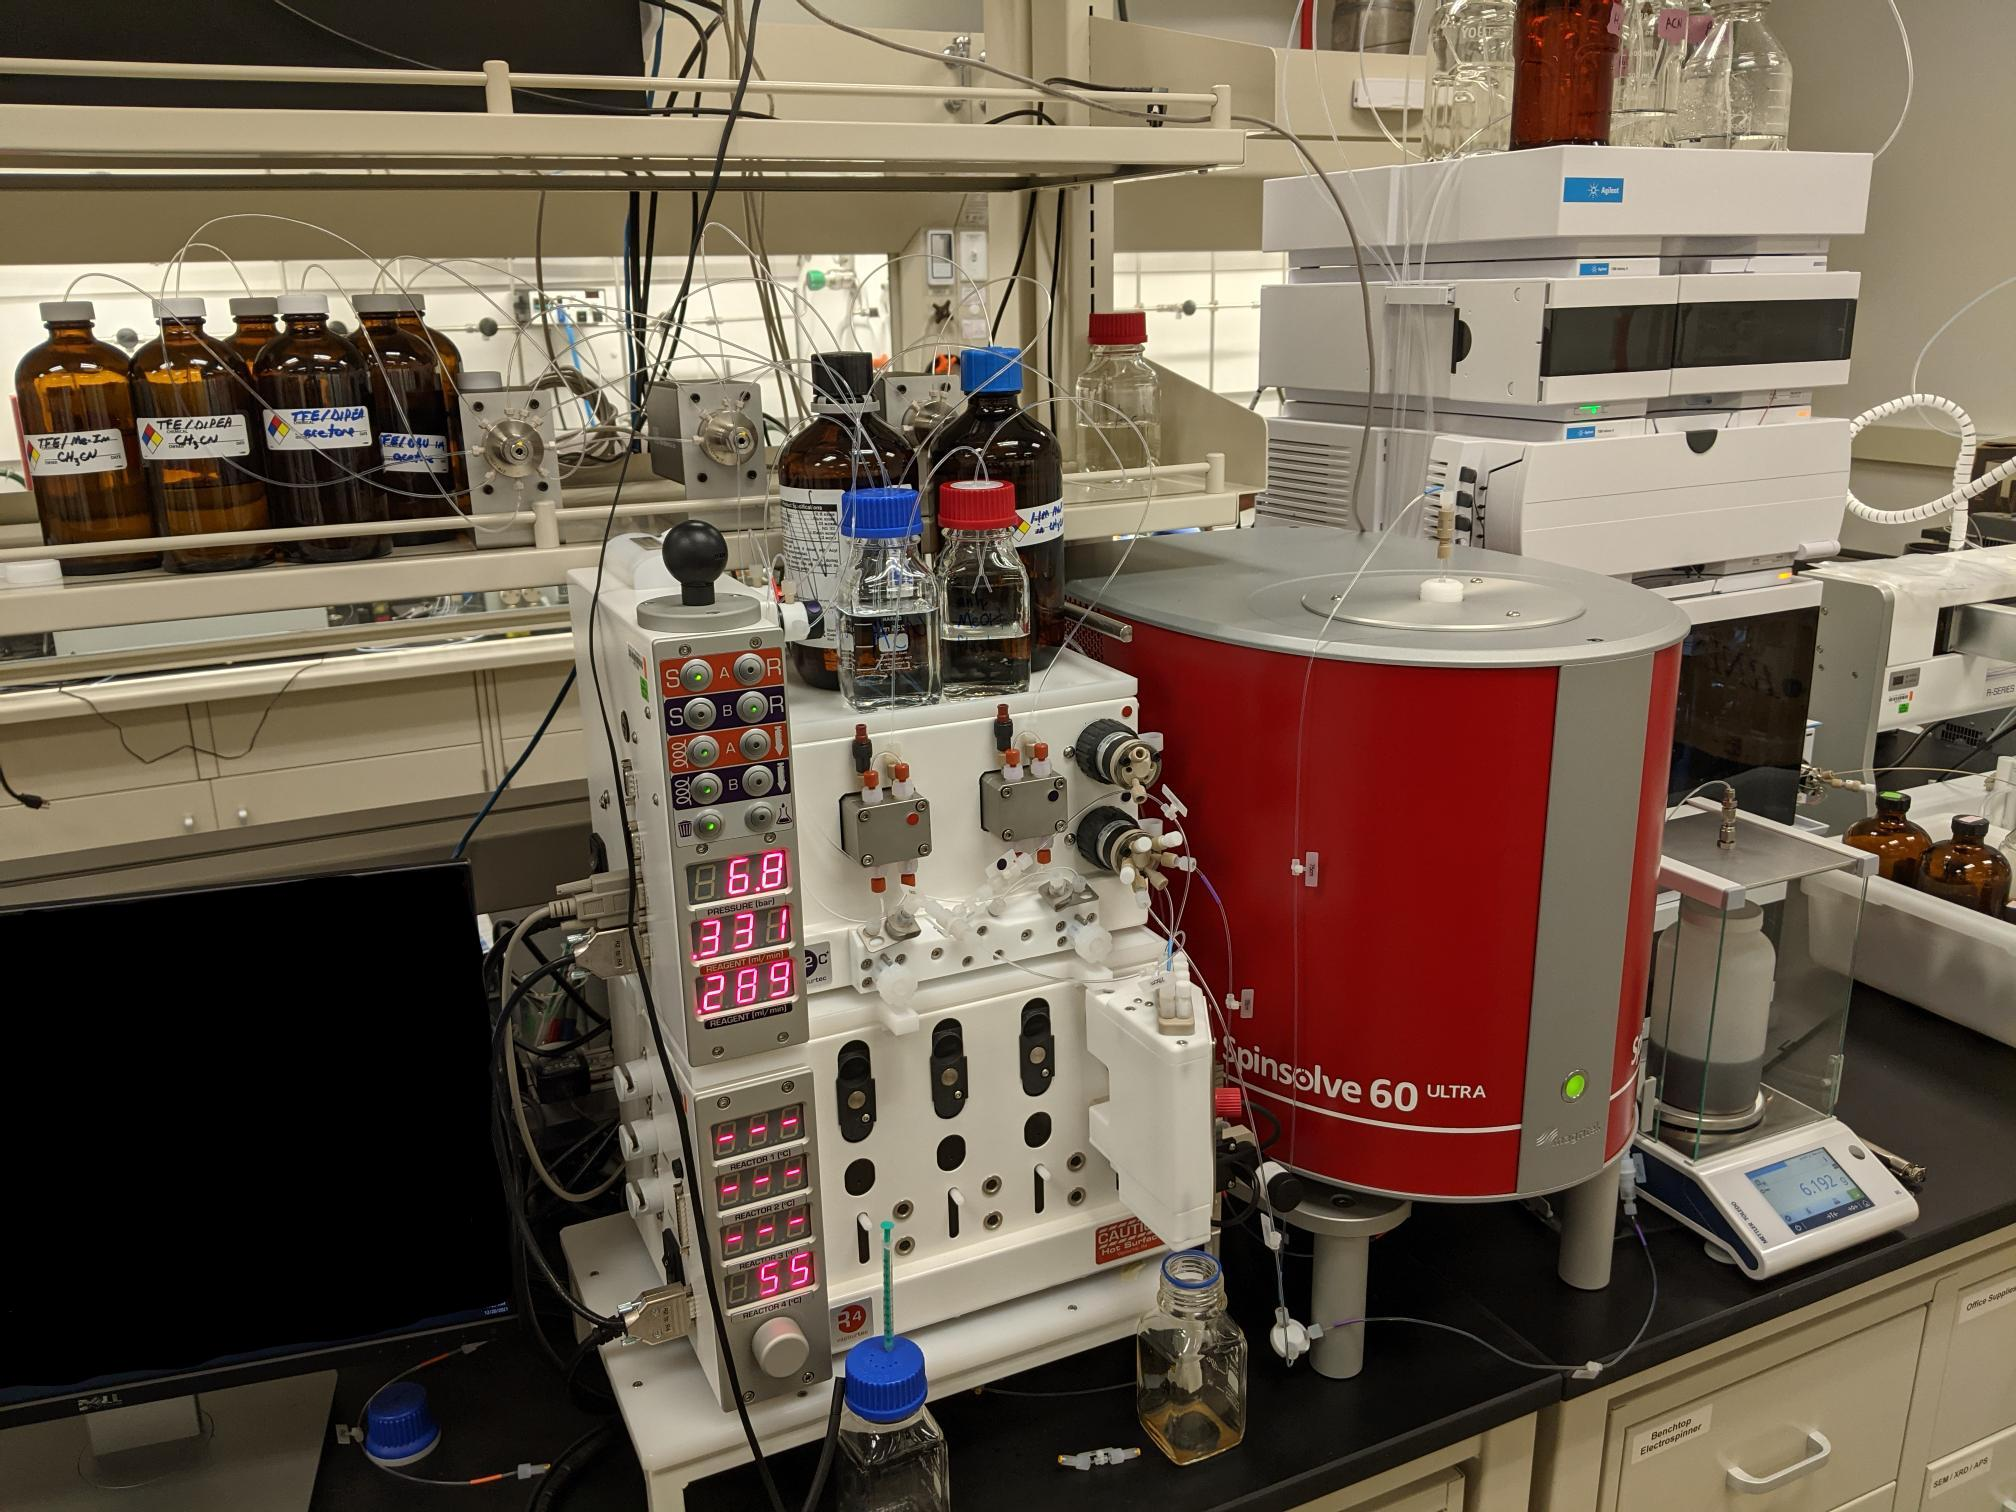
\includegraphics[width=0.38\textwidth]{../img/probs/cfr-nmr-setup.jpg}}
    \hskip -170pt
   \vbox{... in LabVIEW automated CFR\\
    $\quad$ and measured via NMR\\
    $\quad$\\
    Left to right:\\
    PC running LabVIEW\\
    CFR and feed\\
    NMR spectroscope\\}
    }

  }

  \bigskip

  {\small
  {\sl Design variables and bound constraints for experiment}

  \smallskip

      \begin{tabular}{c|cc}
      Parameter & Lower bound & Upper bound \\
      \hline
       Temperature (degrees C) & 40 & 150 \\
       Reaction time (seconds) & 60 & 300 \\
       Equivalence ratio (no units) & 0.9 & 2 \\
  \end{tabular}
  }
  \end{center}
}

%%%%%%%%%%%%%%%%%%%%%%%%%%%%%%%%%%%%%%%%%%%%%%%%%%%%%%%%%%%%%%%%%%%%%%%%%%%%%%
\headerbox{Experiment Results}{name=results,column=2,row=0}{
%%%%%%%%%%%%%%%%%%%%%%%%%%%%%%%%%%%%%%%%%%%%%%%%%%%%%%%%%%%%%%%%%%%%%%%%%%%%%%
  \setlength{\parskip}{0.5\baselineskip}

  \smallskip

  {\small
  \begin{itemize}
  \item {\bf Want to maximize TFMC production at high temperatures}
  \item High temperatures trigger a side-reaction and produces byproduct (TFE)
  \item 15-pt Latin hypercube, Gaussian RBF surrogate, L-BFGS-B optimizer
  \item 3 scalarizations per batch, sorted by temp
  \item evaluated batch on CFR, TFMC and TFE peaks recorded by NMR
  \end{itemize}

  \begin{center}
  {\sl Results after 41 experiments steered by our solver}\\
  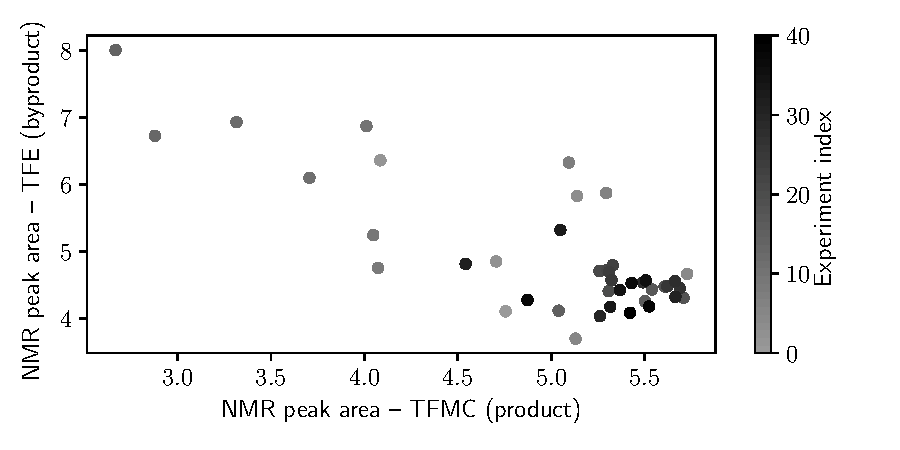
\includegraphics[width=0.7\textwidth]{../img/moo_new/tfmc-tradeoff-eps-converted-to.pdf}\\
  \end{center}

  \vskip -10pt

  {\sl Get this code!}

  {\tt git clone https://github.com/parmoo/cfr-materials\\
  pip install REQUIREMENTS.txt}

  }
}

%%%%%%%%%%%%%%%%%%%%%%%%%%%%%%%%%%%%%%%%%%%%%%%%%%%%%%%%%%%%%%%%%%%%%%%%%%%%%%
\headerbox{Next Steps}{name=future,column=2,below=results}{
%%%%%%%%%%%%%%%%%%%%%%%%%%%%%%%%%%%%%%%%%%%%%%%%%%%%%%%%%%%%%%%%%%%%%%%%%%%%%%
  \setlength{\parskip}{0.5\baselineskip}

  \smallskip
  {\small

  Need to handle more complex design spaces:\\
  \hbox{
  \vbox{
  \begin{itemize}[nosep]
    \item Generative AI for embeddings
    \item Trust-region descent methods
    \item Subspace iterations
  \end{itemize}}
  \hskip -150pt
  \vbox{
  \begin{itemize}[nosep]
    \item Custom surrogate models
    \item Structure-exploiting optimizers
  \end{itemize}}}

  \medskip

  \hbox{
  \vbox{
  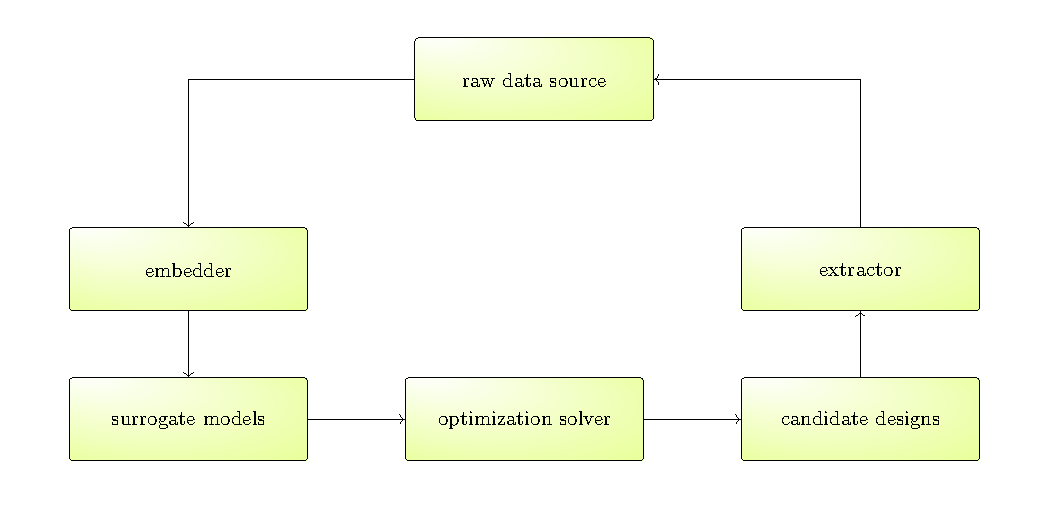
\includegraphics[width=0.55\textwidth]{../img/moo_new/embedder-extractor.pdf}\\
  $\quad$\\
  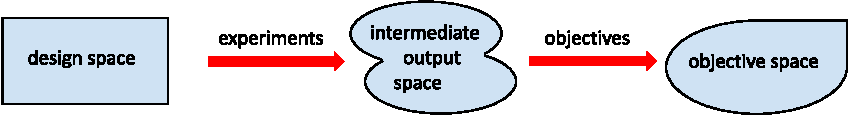
\includegraphics[width=0.6\textwidth]{../img/moo_new/obj-sim-des-space-eps-converted-to.pdf}}
  \hskip -110pt
  \vbox{$\quad$\\
  (Top) using\\
  custom embedders\\
  to optimize in\\
  latent space\\
  $\quad$\\
  (Bottom) exploiting\\
  problem structure\\
  using composite\\
  objectives\\
  }}
  }
}

\begin{posterbox}[name=ack,column=2,below=future,above=bottom,boxheaderheight=0em]
%%%%%%%%%%%%%%%%%%%%%%%%%%%%%%%%%%%%%%%%%%%%%%%%%%%%%%%%%%%%%%%%%%%%%%%%%%%%%%

  {\small

    This material was based upon work supported by the U.S.\ Department of
    Energy, Office of Science, Office of Advanced Scientific Computing
    Research, Applied Mathematics and SciDAC programs under Contract Nos.\
    DE-AC02-05CH11231 and DE-AC02-06CH11357 
    and by the Argonne LDRD program.     

  }
\end{posterbox}

\end{poster}%
%
\end{document}
